%!TEX TS-program = xelatex
%!TEX encoding = UTF-8 Unicode

\documentclass[a4paper, 11pt]{article}

%\newcommand{\LastChange}{Time-stamp: "2014-07-09 15:59:43 aga SeminarProblems.tex"}


% \usepackage[colorinlistoftodos]{todonotes}
\usepackage[colorlinks=true, allcolors=blue]{hyperref}

%\usepackage{euler}
%\usepackage{xltxtra} % loads: fixltx2e, metalogo, xunicode, fontspec

% \usepackage{multicol} % many columns
\usepackage{amsmath,amsfonts,amssymb,amsthm}
\usepackage{fullpage}
\usepackage{graphicx}
\usepackage{bm}
\usepackage{multicol} % текст в несколько колонок

\usepackage{marvosym} % значок мужского туалета

%\usepackage{enumerate}
\usepackage{textcomp} % text in formulas

%\usepackage{paralist}
\usepackage{enumitem} % more options for lists

\usepackage{tikz} % картинки
\usetikzlibrary{arrows.meta, quotes, angles} % tikz-прибамбас для рисовки стрелочек подлиннее

\usepackage[includehead, top=0.5cm, bottom=0.5cm, left=1cm, right=1cm]{geometry}


\usepackage{fontspec} % что-то про шрифты?
\usepackage{polyglossia} % русификация xelatex

\setmainlanguage{russian}
\setotherlanguages{english}

% download "Linux Libertine" fonts:
% http://www.linuxlibertine.org/index.php?id=91&L=1
\setmainfont{Linux Libertine O} % or Helvetica, Arial, Cambria
% why do we need \newfontfamily:
% http://tex.stackexchange.com/questions/91507/
\newfontfamily{\cyrillicfonttt}{Linux Libertine O}

\defaultfontfeatures{Mapping=tex-text}

\AddEnumerateCounter{\asbuk}{\russian@alph}{щ} % для списков с русскими буквами
\setlist[enumerate, 2]{label=\asbuk*),ref=\asbuk*}

%\setmainfont{Times New Roman}
%\setmainfont{Arial}
%\setmainfont{PT Sans}


%\setlength{\topmargin}{0in}
%\setlength{\headheight}{0cm}
%\setlength{\headsep}{0in}
%\setlength{\oddsidemargin}{-0.5in}
%\setlength{\evensidemargin}{-0.5in}
%\setlength{\textwidth}{7.5in}
%\setlength{\textheight}{9.0in}


% \newcommand{\staritem}{\refstepcounter{enumi}\item[\bf *\theenumi.]}

% \newcommand{\bsym}{\boldsymbol}


%\newcommand{\FigWidth}{0.3\columnwidth}



\newtheoremstyle{break}% name
  {}%         Space above, empty = `usual value'
  {1pt}%         Space below
  {}% Body font
  {}%         Indent amount (empty = no indent, \parindent = para indent)
  {\bfseries}% Thm head font
  {.}%        Punctuation after thm head
  {\newline}% Space after thm head: \newline = linebreak
  {}%         Thm head spec

\theoremstyle{break}
\newtheorem{problem}{Задача}[subsection]
\renewcommand{\theproblem}{\arabic{problem}}% Remove subsection from the counter representation


\begin{document}

\thispagestyle{empty}
%%%%%%%%%%%%%%%%%%%%%%%%%%%%%%
%%%%%%%%%%%%%%%%%%%%%%%%%%%%%%
\subsection*{Шестой Тур}
%%%%%%%%%%%%%%%%%%%%%%%%%%%%%%


\begin{problem}
В строй встали 100 граждан Киновии. Они по очереди сделали по одному заявлению.
Начиная со второго все заявления были одинаковые: «Среди сделанных ранее заявлений более 43\% ложных!»

Сколько ложных заявлений сделали эти граждане?
\end{problem}

\begin{problem}
Максимальное расстояние, на которое Адо может метнуть тапок, составляет 80 метров.
На какую максимальную высоту Адо сможет закинуть тапок, метнув его с той же
начальной скоростью?

Дорогой друг, сопротивлением воздуха разрешаю тебе пренебречь! Твой главный судья $\heartsuit$.
\end{problem}


\begin{problem}
Основания трапеции равны $2$ и $10$. Построены вписанная и описанная окружности.
Чему равен радиус описанной окружности?
\end{problem}

\begin{problem}
Блок скатывается с холма высотой $H=5$ м с нулевой начальной скоростью по склону
без трения в сторону точно такого же холма. Между холмами есть горизонтальный участок
$OL$ длиной $L=2$ м и коэффициентом трения $\mu = 0.25$.

На каком расстоянии от основания левого холма (точка $O$) окончательно остановится блок?

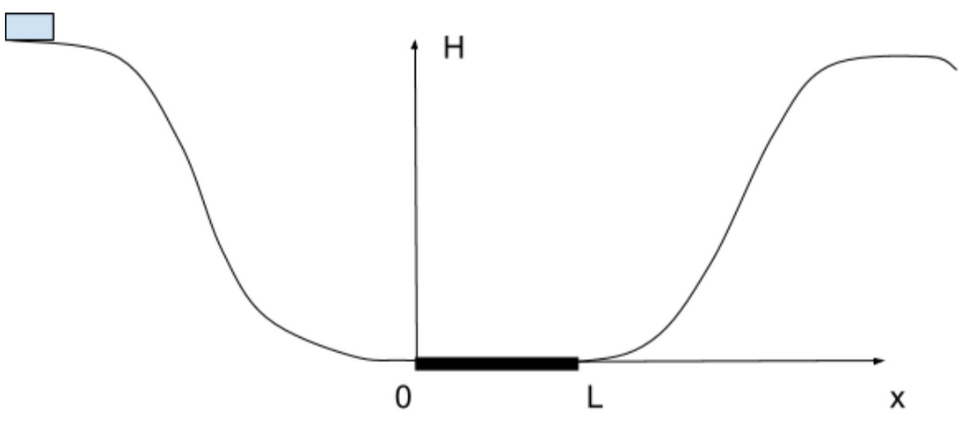
\includegraphics[scale=0.3]{images/6tour_sliding_block.png}
\end{problem}


\subsection*{Шестой Тур}
%%%%%%%%%%%%%%%%%%%%%%%%%%%%%%
\setcounter{problem}{0}


\begin{problem}
В строй встали 100 граждан Киновии. Они по очереди сделали по одному заявлению.
Начиная со второго все заявления были одинаковые: «Среди сделанных ранее заявлений более 43\% ложных!»

Сколько ложных заявлений сделали эти граждане?
\end{problem}

\begin{problem}
Максимальное расстояние, на которое Адо может метнуть тапок, составляет 80 метров.
На какую максимальную высоту Адо сможет закинуть тапок, метнув его с той же
начальной скоростью?

Дорогой друг, сопротивлением воздуха разрешаю тебе пренебречь! Твой главный судья $\heartsuit$.
\end{problem}


\begin{problem}
Основания трапеции равны $2$ и $10$. Построены вписанная и описанная окружности.
Чему равен радиус описанной окружности?
\end{problem}

\begin{problem}
Блок скатывается с холма высотой $H=5$ м с нулевой начальной скоростью по склону
без трения в сторону точно такого же холма. Между холмами есть горизонтальный участок
$OL$ длиной $L=2$ м и коэффициентом трения $\mu = 0.25$.

На каком расстоянии от основания левого холма (точка $O$) окончательно остановится блок?

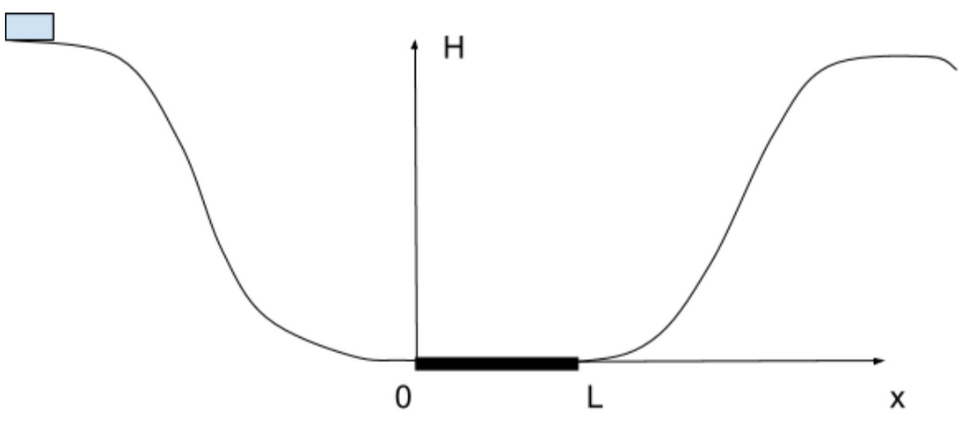
\includegraphics[scale=0.3]{images/6tour_sliding_block.png}
\end{problem}

\end{document}
